\documentclass{article}

\usepackage{final_project,times}
\usepackage{graphicx}
\usepackage{amsmath, amsfonts, amsthm}
\usepackage{enumitem}
\usepackage{xcolor}
\usepackage{hyperref}
\hypersetup{
    colorlinks,
    linkcolor={red!50!black},
    citecolor={blue!50!black},
    urlcolor={blue!80!black}
}
\usepackage{cleveref}

\usepackage{array,tabularx}
\usepackage{subfig}
\usepackage{float}
\restylefloat{table}

% bibliography
\usepackage{natbib}
\bibpunct{(}{)}{;}{a}{}{,} % no comma between author and year

\title{Spike-and-Slab model \& Boosted Tree to Predict Conflict}
\author{Anh Le\\
Department of Political Science\\
Duke University\\
\texttt{anh.le@duke.edu} \\}

\nipsfinalcopy
\begin{document}
\maketitle

\section*{Introduction}

Being able to predict political violence is very useful for governments and international organizations to deploy their limited resources effectively. Traditional models of violence in political science have relied on frequentist panel data methods, which have not had good predictive performance because:

\begin{itemize}[noitemsep]
\item The null hypothesis of $\beta = 0$ being tested is not as important as the substantive effect of the variable
\item Many social science variables are highly correlated. For example, \textit{competitive elections}, \textit{civil liberties}, and \textit{property rights} are three conceptually distinct but empirically correlated variables. This results in (logistic) regression with large coefficient variance and meaningless p-value
\item The problem of collinearity is compounded by the recent explosion of data available, with hundreds of predictors to be considered
\end{itemize}

Therefore, this project will use two methods that work well given the large number of predictors:
\begin{enumerate}
\item sparse regression with spike-and-slab prior
\item (boosted) classification tree
\end{enumerate}

These models are found to perform better than existing models used in our lab.\footnote{We currently use hierarchical linear mixed-effect models, combined together with Bayesian ensemble. The predictors are hand-picked.}

\section{Description of Data}

\textbf{The dataset} contains monthly data of 167 countries from 2001 to present (dimension = $27,000 \times 550$). The training cutoff date is \verb|2013-06-01|.\footnote{This cutoff date is to comply with existing models used in our lab.}

\textbf{The labels} are binary indicators of whether an event happens. We are interested in four types of events: insurgency, rebellion, dpc (domestic political crisis), and erv (ethnic and religious violence), and mp (massive protest).

\textbf{The predictors} include a country's politics, economics, and financial status. I also include spatial lags (constructed from Gower similarity, 4 nearest neighbors, and centroid distance) and temporal lags (by up to 2 months).

\section{Spike-and-Slab}

\subsection{Model building}
I pre-process the data by adding a binary variable that indicates whether an observation belongs to a country. This allows the model to have different intercepts for each country, essentially adding country fixed effect. The spike-and-slab model is fit with the package \verb|BoomSpikeSlab|, running a MCMC chain with $\text{iterations}=5000$ and $\text{burn-in}=500$. 

\subsection{Result}

\autoref{tab:spikeslab_insample} and \autoref{tab:spikeslab_outsample} summarizes the predictive performance of my model. The spike-and-slab model performs well on \verb|insurgency, rebellion, and ethnic violence| (97.6\% precision and 94.6\% recall out of sample), but not well on \verb|domestic crisis| and \verb|massive protest|. \autoref{fig:spikeslab_roc_insurgency} and \autoref{fig:spikeslab_roc_dpc} visualizes this performance discrepancy with ROC curves.

Table \autoref{tab:spikeslab_outsample} and \autoref{tab:ebma_outsample} shows that the spike-and-slab model perform better across labels in comparison with the ensemble model currently used in my lab.

\begin{table}[H]
\centering
% latex table generated in R 3.1.2 by xtable 1.7-4 package
% Mon Dec  8 12:02:52 2014
\begin{tabular}{rrrrrr}
  \hline
 & insurgency & rebellion & dpc & erv & mp \\ 
  \hline
brier & 0.058 & 0.039 & 0.070 & 0.024 & 0.042 \\ 
  auc.C & 0.833 & 0.943 & 0.778 & 0.948 & 0.654 \\ 
  precision & 0.685 & 0.701 & 0.379 & 0.759 & 0.097 \\ 
  recall & 0.529 & 0.566 & 0.064 & 0.477 & 0.007 \\ 
   \hline
\end{tabular}

\caption{In-sample predictive performance}
\label{tab:spikeslab_insample}
\end{table}

\begin{table}[H]
\centering
\subfloat[Spike-and-Slab]{\label{tab:spikeslab_outsample}
	% latex table generated in R 3.1.2 by xtable 1.7-4 package
% Mon Dec  8 12:02:52 2014
\begin{tabular}{rrrrrr}
  \hline
 & insurgency & rebellion & dpc & erv & mp \\ 
  \hline
brier & 0.080 & 0.057 & 0.167 & 0.037 & 0.049 \\ 
  auc.C & 0.886 & 0.895 & 0.688 & 0.922 & 0.704 \\ 
  precision & 0.519 & 0.575 & 0.162 & 0.508 & 0.097 \\ 
  recall & 0.778 & 0.586 & 0.458 & 0.504 & 0.033 \\ 
   \hline
\end{tabular}
}
\subfloat[Ensemble Linear Mixed Effect]{\label{tab:ebma_outsample}
	\begin{tabular}{rrrrr}
  \hline
 & insurgency & rebellion & dpc & erv \\ 
  \hline
brier & 0.06 & 0.03 & 0.12 & 0.03 \\ 
  auc.C & 0.94 & 0.97 & 0.78 & 0.93 \\ 
   \hline
\end{tabular}}
\caption{Table \autoref{tab:spikeslab_outsample} shows the out-sample performance of the Spike-and-Slab model, which performs better (according to Brier and AUC score) than the currently used Ensemble model in Table \autoref{tab:ebma_outsample}}
\end{table}

\begin{figure}[H]
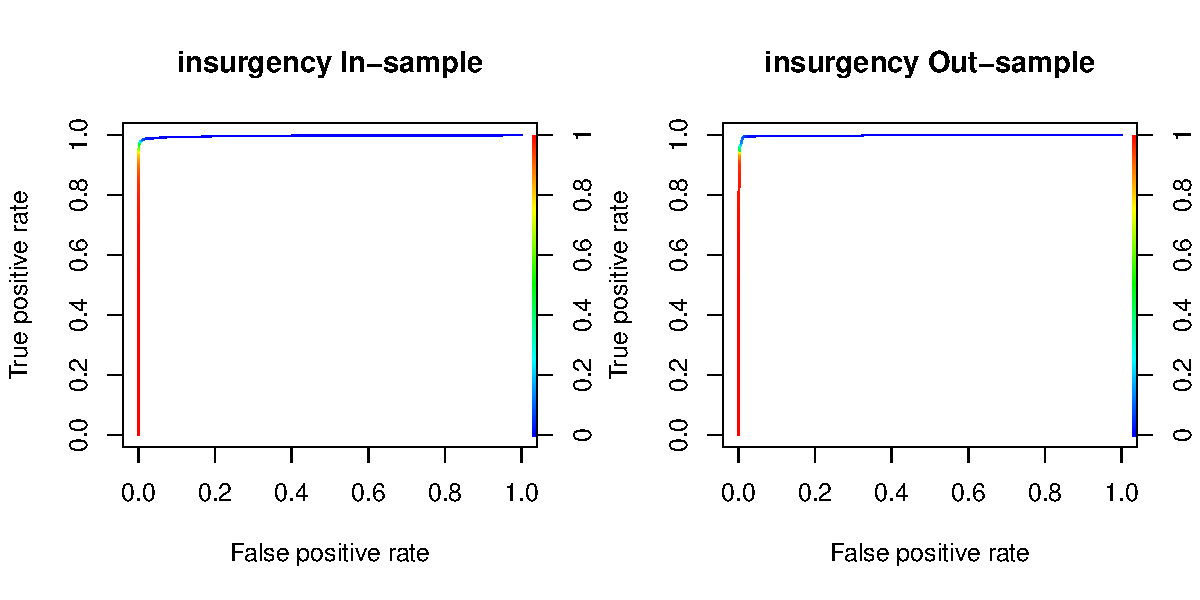
\includegraphics[width=\textwidth]{fig/spikeslab_roc_insurgency}
\caption{ROC curve of insurgency prediction}
\label{fig:spikeslab_roc_insurgency}
\end{figure}

\begin{figure}[H]
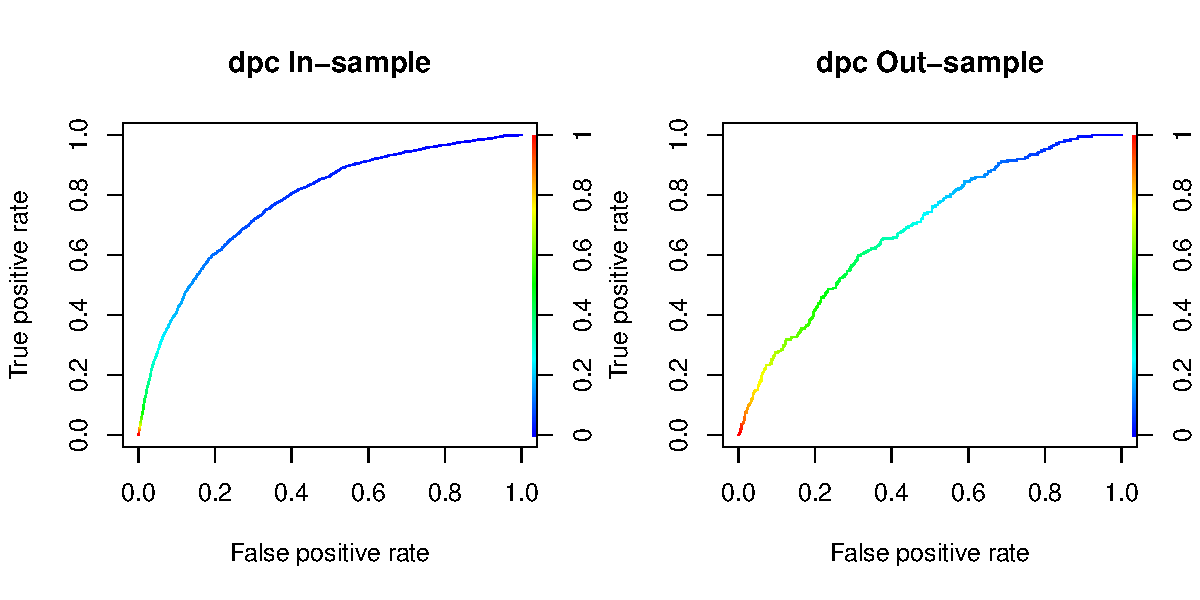
\includegraphics[width=\textwidth]{fig/spikeslab_roc_dpc}
\caption{ROC curve of domestic crisis prediction}
\label{fig:spikeslab_roc_dpc}
\end{figure}

However, looking at \autoref{fig:spikeslab_insurgencyvar}, it becomes clear that most of the predictive performance comes from the country dummies. This is because some countries almost always experience insurgency, while some other countries almost never, so it is safe to predict that these countries will follow the same pattern in the future. Therefore, even though the model has excellent performance, it is not necessarily revealing important factors that predict insurgency.

\begin{figure}[H]

\includegraphics[width=\textwidth]{fig/spikeslab_insurgencyvar}
\caption{The left figure lists all the variables. The spike-and-slab model selects only a very small subset of the predictors. The right figure lists the variables with inclusion probability larger than 0.001. The majority of these predictors are country dummies.}
\label{fig:spikeslab_insurgencyvar}
\end{figure}

Indeed, \autoref{tab:withhier_vs_nohier_spikeslab} shows that the model performance deteriorates sharply without the country dummies. \autoref{fig:nohierspikeslab_insurgencyvar} shows the variables selected when there is no country dummy. Many more interesting predictive factors are revealed, such as the number opposition resistance events in neighboring countries, infant mortality rate, international tourism, etc.

\begin{table}[H]
\centering
\begin{tabular}{c}
\subfloat[With country dummies]{\label{tab:withhierspikeslab_outsample}
	% latex table generated in R 3.1.2 by xtable 1.7-4 package
% Mon Dec  8 12:02:52 2014
\begin{tabular}{rrrrrr}
  \hline
 & insurgency & rebellion & dpc & erv & mp \\ 
  \hline
brier & 0.080 & 0.057 & 0.167 & 0.037 & 0.049 \\ 
  auc.C & 0.886 & 0.895 & 0.688 & 0.922 & 0.704 \\ 
  precision & 0.519 & 0.575 & 0.162 & 0.508 & 0.097 \\ 
  recall & 0.778 & 0.586 & 0.458 & 0.504 & 0.033 \\ 
   \hline
\end{tabular}
}\\
\subfloat[Without country dummies]{\label{tab:nohierspikeslab_outsample}
	% latex table generated in R 3.1.2 by xtable 1.7-4 package
% Mon Dec  8 18:36:13 2014
\begin{tabular}{rrrrrr}
  \hline
 & insurgency & rebellion & dpc & erv & mp \\ 
  \hline
brier & 0.080 & 0.057 & 0.167 & 0.037 & 0.049 \\ 
  auc.C & 0.886 & 0.895 & 0.688 & 0.922 & 0.704 \\ 
  precision & 0.519 & 0.575 & 0.162 & 0.508 & 0.097 \\ 
  recall & 0.778 & 0.586 & 0.458 & 0.504 & 0.033 \\ 
   \hline
\end{tabular}
}
\end{tabular}
\caption{Table \autoref{tab:nohierspikeslab_outsample} shows the out-sample performance of the Spike-and-Slab model without country dummies, which performs much worse.}
\label{tab:withhier_vs_nohier_spikeslab}
\end{table}

\begin{figure}[H]
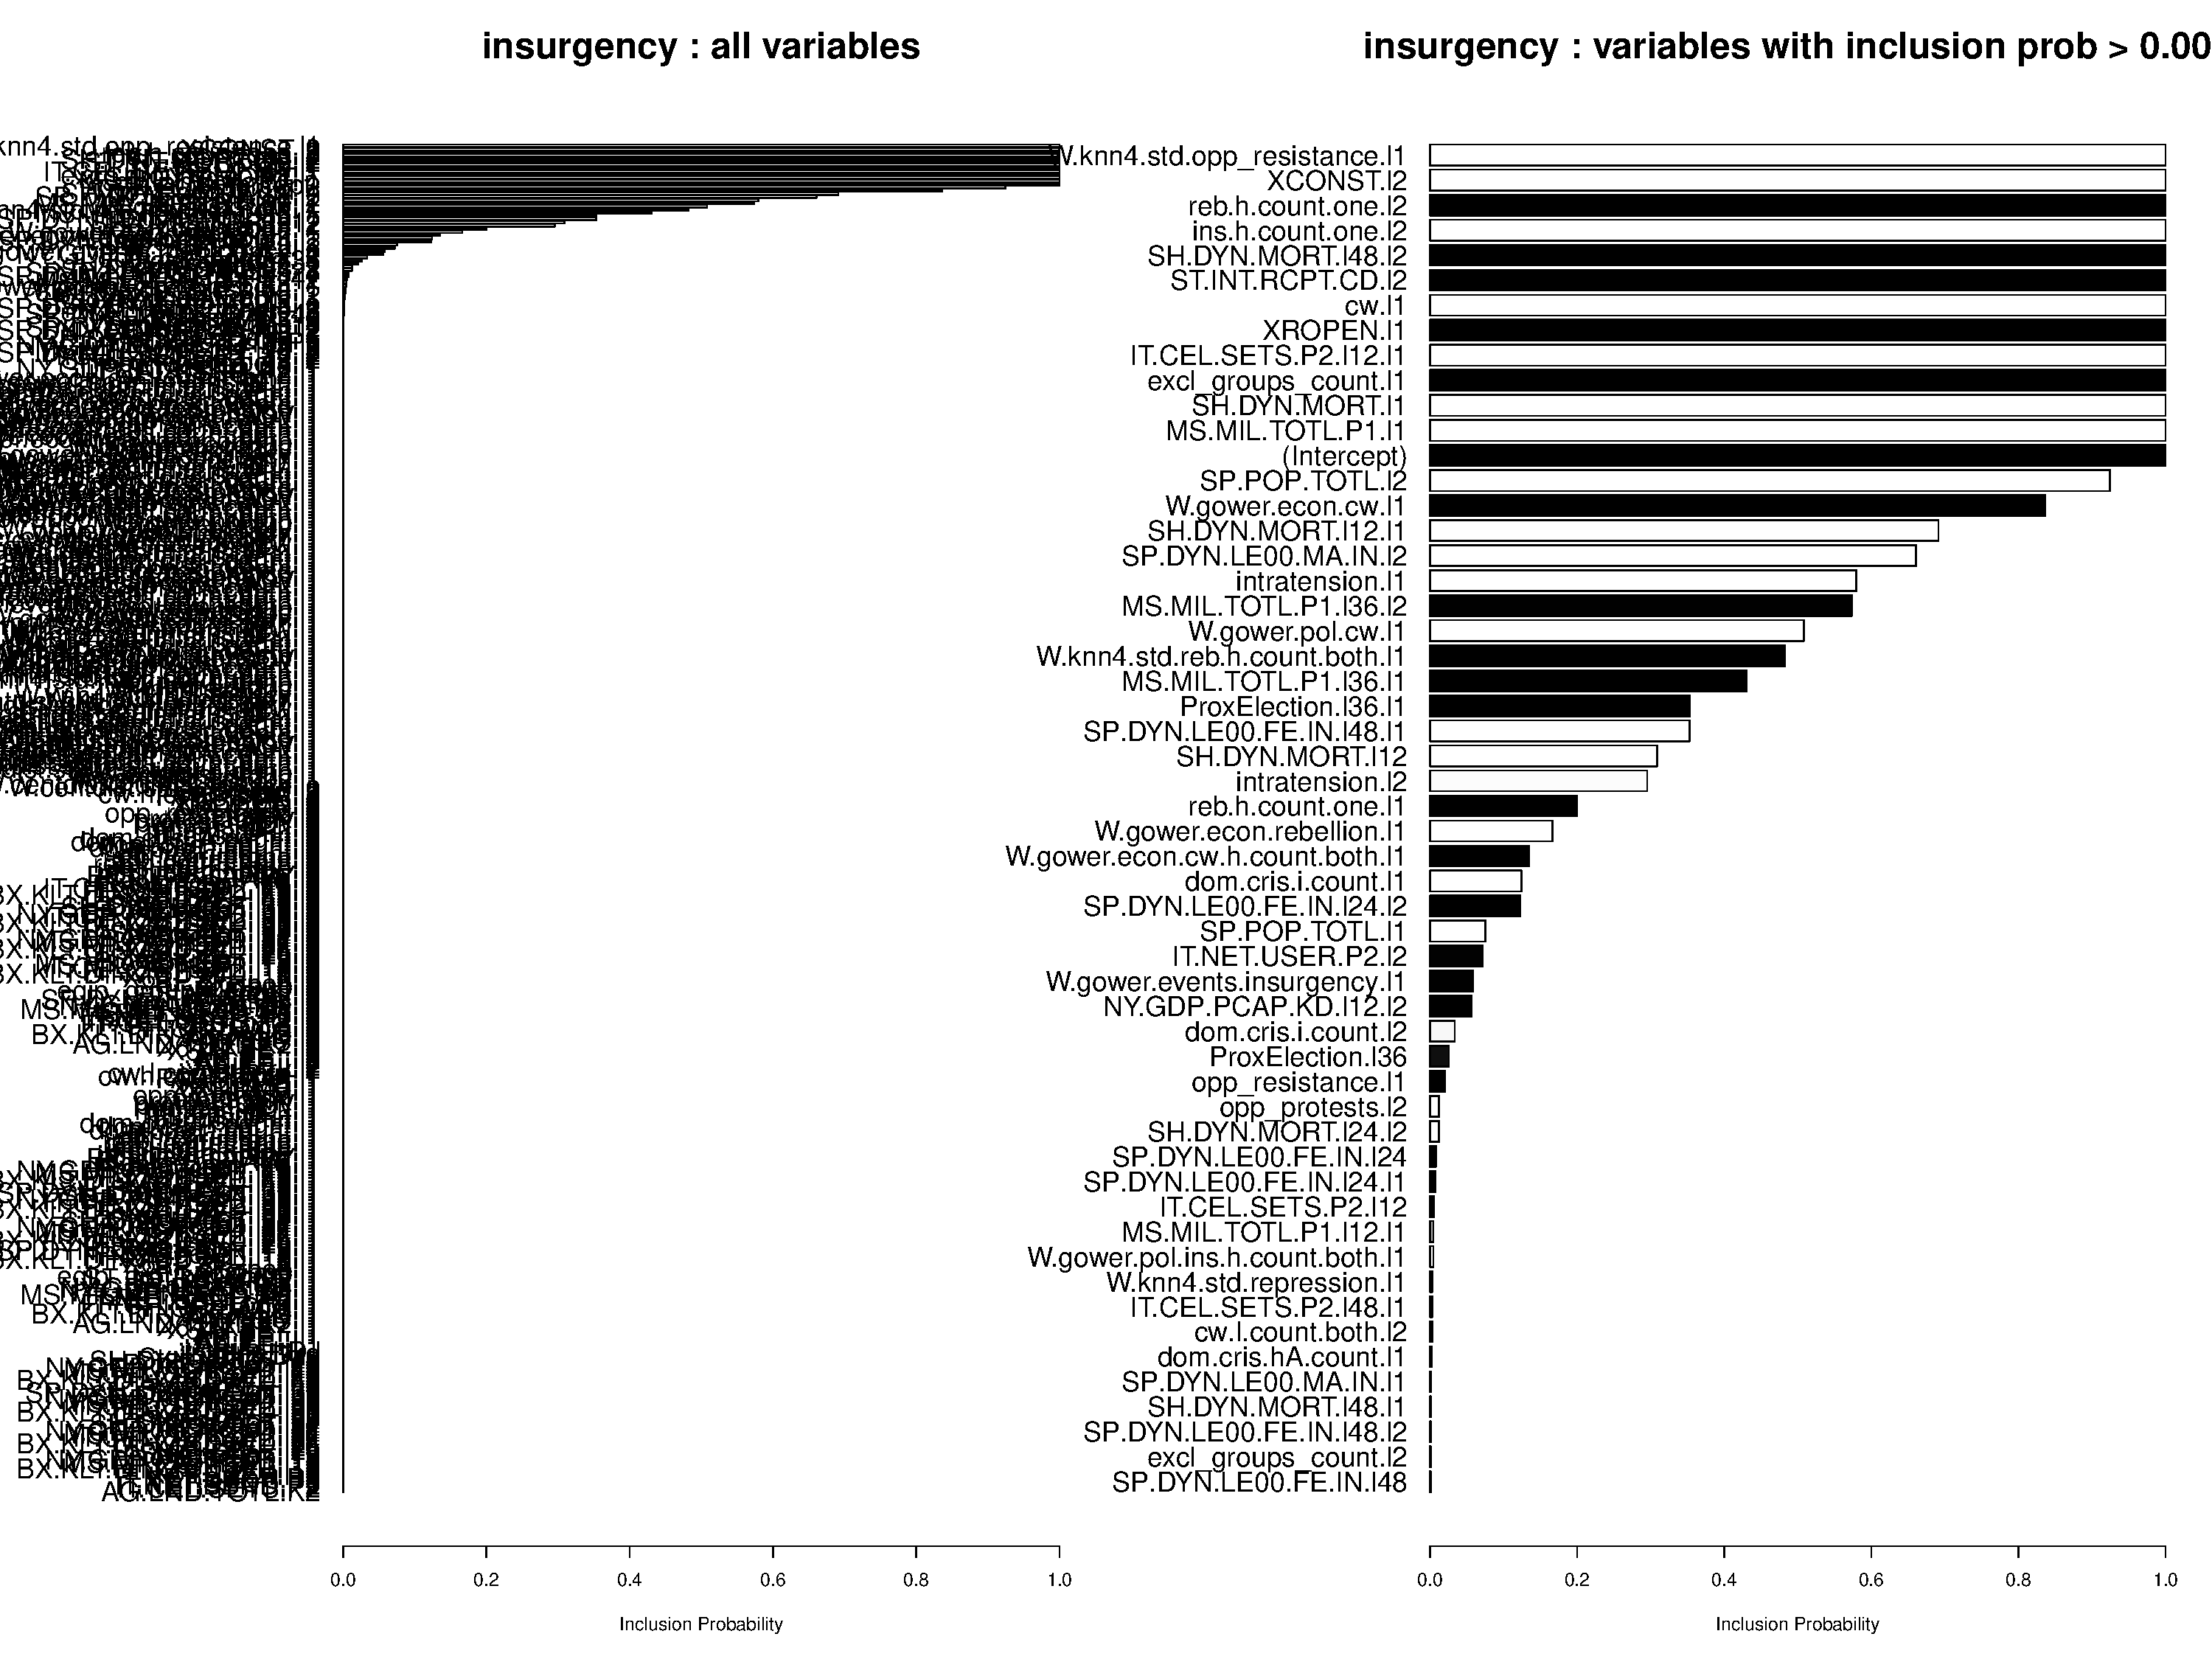
\includegraphics[width=\textwidth]{fig/nohierspikeslab_insurgencyvar}
\caption{Variable Selection when there is no country dummies}
\label{fig:nohierspikeslab_insurgencyvar} 
\end{figure}

\section{Tree-based model}

\subsection{Model building}

Since the spike-and-slab model does not work well without country dummies, in this section I will try tree-based model. From now on, I will also use a month's predictors to predict \textit{next month}'s event instead.\footnote{I am not sure why our lab is ``predicting'' a month's event with the predictors of the current month. This seems to defeat the purpose of predicting conflict in advance in order to better prepare for it.}

\begin{itemize}[noitemsep]
\item Classification tree with pruning via cross-validation
\item Boosted tree, with 
\begin{itemize}[noitemsep]
\item \text{tree.complexity} = 1
\item learning.rate = 0.01
\item bag.fraction = 0.75	
\item 10-fold cross-validation
\end{itemize}
\end{itemize}

\subsection{Classification tree result}

Table \autoref{tab:cart_in_sample} and \autoref{tab:cart_out_sample} show the predictive performance of pruned tree. There is not much improvement over spike-and-slab model. \autoref{fig:insurgency_tree} shows the decision tree for predicting insurgency.							

\begin{table}[!ht]
\centering
\begin{tabular}{c}
\subfloat[In-Sample]{\label{tab:cart_in_sample}
	% latex table generated in R 3.1.2 by xtable 1.7-4 package
% Mon Dec  8 18:48:30 2014
\begin{tabular}{rrrrr}
  \hline
 & insurgency & rebellion & dpc & erv \\ 
  \hline
precision & 0.680 & 0.693 & 0.605 & 0.823 \\ 
  recall & 0.665 & 0.784 & 0.064 & 0.713 \\ 
   \hline
\end{tabular}
}\\
\subfloat[Out-Sample]{\label{tab:cart_out_sample}
	% latex table generated in R 3.1.2 by xtable 1.7-4 package
% Mon Dec  8 18:48:30 2014
\begin{tabular}{rrrrr}
  \hline
 & insurgency & rebellion & dpc & erv \\ 
  \hline
precision & 0.614 & 0.600 & 0.148 & 0.820 \\ 
  recall & 0.713 & 0.606 & 0.042 & 0.575 \\ 
   \hline
\end{tabular}
}
\end{tabular}
\caption{In- and Out-Sample performance of decision tree}
\end{table}

\begin{figure}[!ht]
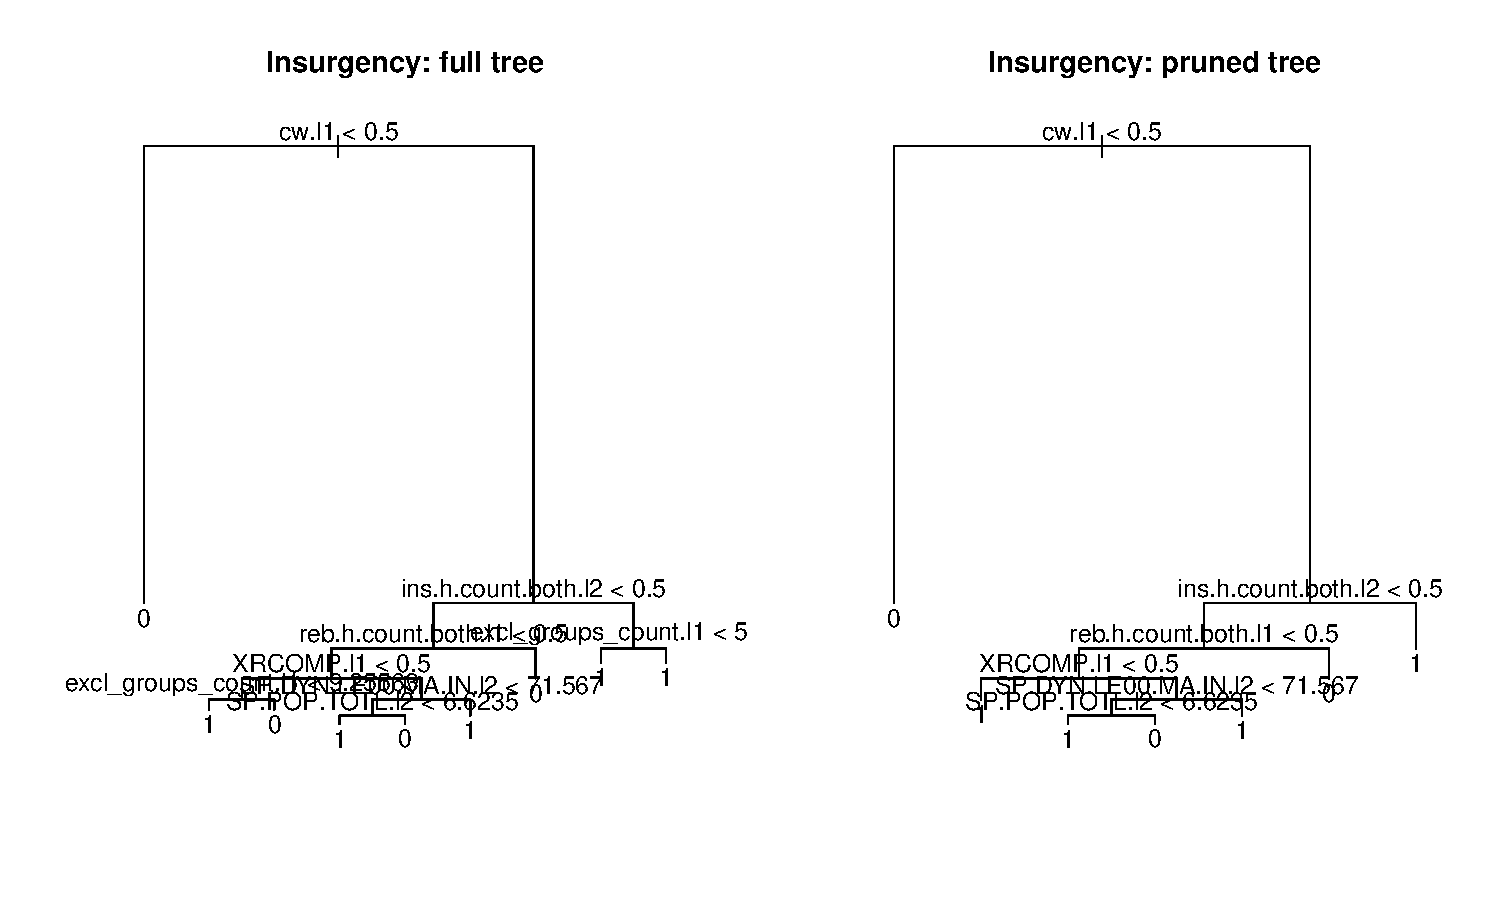
\includegraphics[width=\textwidth]{fig/insurgency_tree}
\caption{The decision tree to predict insurgency. Left: full tree. Right: pruned tree}
\label{fig:insurgency_tree}
\end{figure}

\subsection{Boosted tree result}

Table \autoref{tab:boosting_insample} and \autoref{tab:boosting_outsample} shows the predictive performance of boosted classification tree, which is substantially better than individual tree. The precision and recall improves by 15 - 30 \% for \verb|insurgency, rebellion, ethnic violence|. Most dramatically is the improvement in prediction for \verb|domestic crisis|, which goes from 14\% to 65\% in precision, and from 4.2\% to 22\% in recall.

\begin{table}[!ht]
\centering
\begin{tabular}{c}
\subfloat[In-Sample]{\label{tab:boosting_insample}
	% latex table generated in R 3.1.2 by xtable 1.7-4 package
% Wed Feb 11 15:42:07 2015
\begin{tabular}{rrrrrr}
  \hline
 & insurgency & rebellion & dpc & erv & mp \\ 
  \hline
brier & 0.006 & 0.005 & 0.039 & 0.031 & 0.033 \\ 
  auc.C & 0.997 & 0.999 & 0.946 & 0.980 & 0.857 \\ 
  precision & 0.971 & 0.965 & 0.705 & 0.542 & 0.541 \\ 
  recall & 0.964 & 0.968 & 0.521 & 0.926 & 0.118 \\ 
   \hline
\end{tabular}
}\\
\subfloat[Out-Sample]{\label{tab:boosting_outsample}
	% latex table generated in R 3.1.1 by xtable 1.7-3 package
% Sun Jan 25 23:20:49 2015
\begin{tabular}{rrrrr}
  \hline
 & insurgency & rebellion & dpc & erv \\ 
  \hline
brier & 0.008 & 0.012 & 0.091 & 0.037 \\ 
  auc.C & 0.996 & 0.984 & 0.899 & 0.956 \\ 
  precision & 0.971 & 0.958 & 0.584 & 0.659 \\ 
  recall & 0.963 & 0.854 & 0.730 & 0.712 \\ 
   \hline
\end{tabular}
}
\end{tabular}
\caption{In- and Out-Sample predictive performance of Boosted Classification Tree}
\end{table}

\section{Conclusion}

In this project I predict conflict event with two methods that work well in high-dimensional data: 1) Spike-and-Slab variable selection, and 2) (Boosted) Classification Tree. In both cases, out-sample predictive performance is only slightly worse than in-sample performance, suggesting that the two method successfully avoid overfitting.

The Spike-and-Slab model also reveals the important factor of country dummies in predicting conflict event. It shows that the existing models have excellent performance (up to 97\% precision and 94\% recall on \verb|insurgency|) simply because some countries always (never) have conflict events. Once the country dummies are taken out, the Spike-and-Slab model performs much worse.

Finally, when there is no country dummy, (boosted) classification tree performs substantially better than single tree and spike-and-slab model.
\end{document}
